\subsection{Cellular Automata}

\begin{itemize}
    \item What is a Cellular Automata?
    \item Turing-complete CA with 29 states \cite{neumann1966selfreplication}.
    \item Codd: Turing-complete CA with 8 states, given some conditions \cite{codd1968cellular}
    \item Langton's research on emergent computation and phase transition \cite{langton1990edgeofchaos}.
    \item Wolfram's four qualitative CA classes \cite{wolfram1984complexity}?
\end{itemize}

\subsection{Self-Replication}

\begin{itemize}
    \item von Neumann's work on self-replication from around 1950 \cite{neumann1966selfreplication}.
    \item Self-replicating structures \cite{reggia1998neumann}
    \item Replicating universal computers with 63 states and 8500 rules \cite{perrier1996toward}.
\end{itemize}

\subsection{Evolution}

\begin{itemize}
    \item Genetic Algorithms
    \item Evolution in materio/silicon \cite{miller2014evolution}
\end{itemize}

\subsection{Artificial Development}

\begin{itemize}
    \item \cite{harding2008artificial} \cite{tufte2008evodevo}
    \item Zygote
    \item Scalability
    \item Robustness
    \item Plasticity
\end{itemize}

\subsection{Sblock: Haddow}

\begin{itemize}
    \item \cite{haddow2000sblock}
    \item Sblock
\end{itemize}

\subsection{FPGA}

\begin{figure}[!ht]
    \centering
    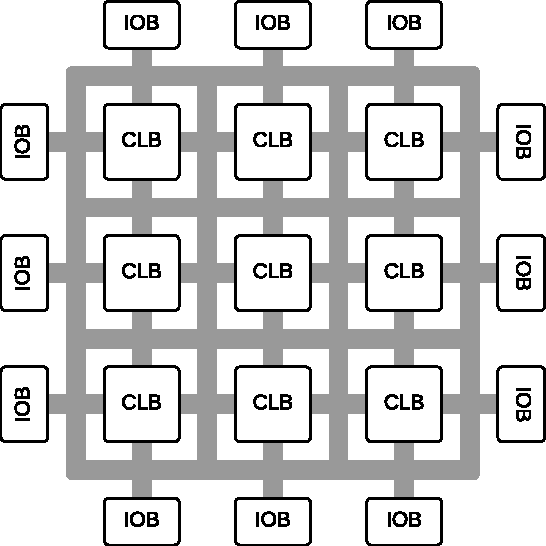
\includegraphics[width=0.30\textwidth]{figures/fpga}
    \caption{High-level block diagram of an FPGA. An array of configurable logic blocks (CLBs) and input/output blocks (IOBs) are connected by a network of interconnects.}
    \label{fig:overview-aamodt}
\end{figure}

\TODO

\subsection{Energy/Parallel}

\TODO

